%\documentclass[
%  paper=a4,
%  fontsize=11pt,
%  DIV=12,
%  parskip=half,
%  headings=big,
%  numbers=noenddot,
%  twoside=false
%]{scrbook}
%
%\usepackage[ngerman]{babel}
%\usepackage{csquotes}
%\usepackage{microtype}
%\usepackage{booktabs}
%\usepackage{tikz}
%\usepackage{pgfplots}
%\pgfplotsset{
%  compat=1.18,
%  every axis/.append style={font=\small},
%}
%\usepackage[firafull]{addfonts}
%\usepackage{scrlayer-scrpage}
%\usepackage[hidelinks]{hyperref}
%
%\pagestyle{scrheadings}
%\clearpairofpagestyles
%
%\ihead{}
%\ohead{\chaptermark}
%\chead{}
%
%\ofoot[\pagemark]{\pagemark}
%\cfoot{}
%\makeatletter
%\ifoot[\textcolor{gray!40}{\footnotesize © \the\year\ \@author}]{\textcolor{gray!40}{\footnotesize © \the\year\ \@author}}
%\makeatother
%
%\automark{chapter}

\documentclass[
]{bfbook}


\title{Modernes Textsatzsystem\\Grundlagen, Werkzeuge und Praxis}
\author{Benno Falkner}
\date{\today}



\begin{document}

\frontmatter
\maketitle
\tableofcontents

\chapter{Vorwort}

Typografie ist keine Dekoration — sie ist Kommunikation. Ein gut gesetzter
Text erleichtert das Lesen, strukturiert Gedanken und gibt einem Dokument
Haltung. Dieses Buch führt in die Werkzeuge ein, die professionellen
Textsatz auf einem Computer ermöglichen: \TeX, \LaTeX\ und KOMA-Script.

Die Quellen dieses Buches sind drei Werke, die zusammen das Fundament
der \TeX-Welt bilden: Knuths \emph{TeXbook}~\cite{knuth1984texbook},
der \emph{LaTeX Companion}~\cite{mittelbach2004latex} und Kohms
\emph{KOMA-Script}~\cite{kohm2021komascript}.

\mainmatter

\chapter{Die Geschichte des Textsatzes}

\section{Vor \TeX}

Vor der Entwicklung von \TeX\ war professioneller Textsatz ein handwerklicher
Beruf. Bleilettern wurden von Hand gesetzt, Abstände mit Spatien gefüllt,
Seiten in Rahmen gespannt und auf der Druckpresse vervielfältigt. Die
Einführung des Fotosatzes in den 1960er Jahren mechanisierte diesen Prozess,
löste aber das grundlegende Problem nicht: die Qualität des Satzes hing
vom Geschick des Setzers ab.

\section{Donald Knuth und die Geburt von \TeX}

Donald Knuth entwickelte \TeX\ ab 1977 aus Unzufriedenheit mit der
typografischen Qualität seiner eigenen Bücher. Sein Ziel war ein System,
das mathematisch präzisen, ästhetisch überzeugenden Textsatz automatisch
erzeugt~\cite{knuth1984texbook}.

Das Ergebnis war revolutionär: \TeX\ behandelt Textsatz als
Optimierungsproblem. Der Zeilenumbruchalgorithmus von Knuth und Plass
minimiert eine globale Strafunktion $\mathcal{P}$:

\[
  \mathcal{P} = \sum_{i} \left( r_i^3 + p_i \right)
\]

wobei $r_i$ das Streckungsverhältnis der $i$-ten Zeile und $p_i$ die
Strafe für Trennungen und andere unerwünschte Brüche bezeichnet. Dieser
Ansatz unterscheidet \TeX\ fundamental von greedy-basierten Algorithmen,
die Zeile für Zeile entscheiden.

\section{Von \TeX\ zu \LaTeX}

Leslie Lamport entwickelte Anfang der 1980er Jahre \LaTeX\ als Makropaket
auf Basis von \TeX. Während \TeX\ ein Programmiersystem ist, bietet \LaTeX\
vorgefertigte Strukturen: Dokumentklassen, Umgebungen, Querverweise und
Bibliografien~\cite{mittelbach2004latex}.

Tabelle~\ref{tab:vergleich} zeigt die wichtigsten Unterschiede zwischen
den Systemen.

\begin{table}[h]
\centering
\caption{Vergleich der Textsatzsysteme}
\label{tab:vergleich}
\begin{tabular}{llll}
\toprule
System & Ebene & Stärke & Typischer Einsatz \\
\midrule
Plain \TeX   & Primitiv    & maximale Kontrolle  & Bücher, Spezialformate \\
\LaTeX       & Makros      & Struktur            & Wissenschaft, Technik \\
KOMA-Script  & Klassen     & Europäische Normen  & Briefe, Berichte \\
Tectonic     & Engine      & moderne Fonts       & portable Builds \\
\bottomrule
\end{tabular}
\end{table}

\chapter{Typografie und Algorithmen}

\section{Zeilenumbruch als Optimierung}

Der Knuth-Plass-Algorithmus betrachtet einen ganzen Absatz als Einheit.
Er sucht die Menge von Zeilenbrüchen $B = \{b_1, b_2, \ldots, b_n\}$,
die die Gesamtstrafe minimiert. Im Gegensatz zu greedy-Algorithmen kann
er eine schlechte Zeile in Kauf nehmen, um den Absatz insgesamt besser
zu machen.

Abbildung~\ref{fig:penalty} zeigt schematisch wie die Strafwerte mit
dem Streckungsverhältnis wachsen.

\begin{figure}[h]
\centering
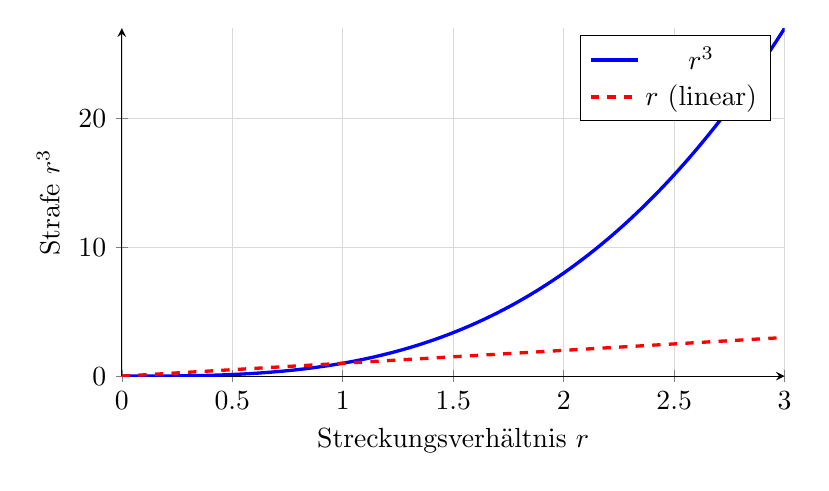
\begin{tikzpicture}
\begin{axis}[
  width=10cm,
  height=6cm,
  xlabel={Streckungsverhältnis $r$},
  ylabel={Strafe $r^3$},
  axis lines=left,
  xmin=0, xmax=3,
  ymin=0, ymax=27,
  grid=major,
  grid style={line width=0.2pt, draw=gray!30},
  every axis plot/.append style={line width=1.2pt},
]
\addplot[blue, domain=0:3, samples=100] {x^3};
\addlegendentry{$r^3$}
\addplot[red, dashed, domain=0:3, samples=100] {x};
\addlegendentry{$r$ (linear)}
\end{axis}
\end{tikzpicture}
\caption{Kubische Straffunktion des Knuth-Plass-Algorithmus}
\label{fig:penalty}
\end{figure}

\section{Mikrotypografie}

Das Paket \texttt{microtype} aktiviert mikrotypografische Erweiterungen
die \TeX\ allein nicht bietet: \emph{character protrusion} lässt
Satzzeichen leicht in den Rand hineinragen, \emph{font expansion} streckt
und staucht Schriftzeichen minimal um den Zeilenumbruch zu verbessern.

Der Effekt ist subtil aber messbar — Absätze mit \texttt{microtype} haben
im Durchschnitt weniger Trennungen und gleichmäßigere Grauwerte.

\section{Schrifttechnologie}

Moderne \TeX-Engines wie XeTeX und LuaTeX unterstützen OpenType-Schriften
direkt über das Paket \texttt{fontspec}. OpenType-Schriften kodieren
typografische Intelligenz direkt in der Schriftdatei: Ligaturen,
Kerning-Tabellen, optische Größen und variable Achsen.

Tabelle~\ref{tab:fontfeatures} listet die wichtigsten OpenType-Features.

\begin{table}[h]
\centering
\caption{OpenType-Features im Überblick}
\label{tab:fontfeatures}
\begin{tabular}{ll}
\toprule
Feature & Beschreibung \\
\midrule
Ligaturen        & Verschmelzung von Buchstabenpaaren (fi, fl, ff) \\
Kerning          & Zeichenabstand zwischen Paaren \\
Optische Größen  & Schriftoptimierung je nach Schriftgröße \\
Variable Fonts   & Kontinuierliche Achsen für Gewicht, Breite etc. \\
Oldstyle-Ziffern & Ziffern mit Ober- und Unterlängen \\
\bottomrule
\end{tabular}
\end{table}

\chapter{KOMA-Script}

\section{Europäische Typografie}

Die Standardklassen von \LaTeX\ — \texttt{article}, \texttt{book},
\texttt{letter} — folgen amerikanischen typografischen Konventionen.
KOMA-Script ersetzt diese durch europäisch orientierte Klassen:
\texttt{scrartcl}, \texttt{scrbook}, \texttt{scrlttr2}~\cite{kohm2021komascript}.

Die Unterschiede sind nicht kosmetisch. DIN~5008 regelt den deutschen
Geschäftsbrief bis ins Detail: Faltmarken, Rücksenderzeile, Adressfeld,
Betreffzeile. \texttt{scrlttr2} implementiert diese Norm vollständig
und konfigurierbar.

\section{Das Typenmaß-System}

KOMA-Script verwendet das \texttt{DIV}-System zur Seitenaufteilung.
Der Parameter \texttt{DIV} teilt die Seite in $n \times n$ Einheiten
und legt daraus Satzspiegel und Ränder fest. Für \texttt{DIV=12} ergibt
sich ein Satzspiegel der $\frac{10}{12}$ der Seitenbreite und
$\frac{10}{12}$ der Seitenhöhe einnimmt.

\begin{figure}[h]
\centering
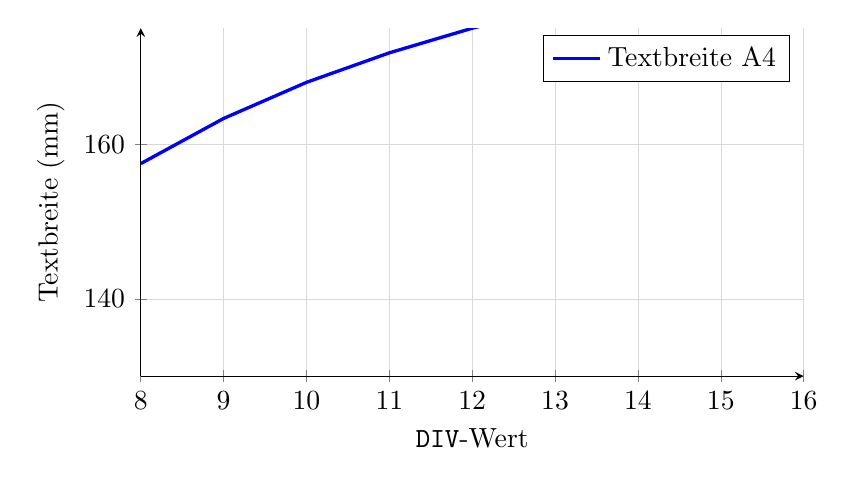
\begin{tikzpicture}
\begin{axis}[
  width=10cm,
  height=6cm,
  xlabel={\texttt{DIV}-Wert},
  ylabel={Textbreite (mm)},
  axis lines=left,
  xmin=8, xmax=16,
  ymin=130, ymax=175,
  grid=major,
  grid style={line width=0.2pt, draw=gray!30},
  every axis plot/.append style={line width=1.2pt},
  xtick={8,9,10,11,12,13,14,15,16},
]
\addplot[blue, domain=8:16, samples=9] {210*(x-2)/x};
\addlegendentry{Textbreite A4}
\end{axis}
\end{tikzpicture}
\caption{Textbreite in Abhängigkeit vom \texttt{DIV}-Wert auf A4}
\end{figure}

\chapter{Modernes \TeX\ mit Tectonic}

\section{Das Problem klassischer Distributionen}

TeXLive und MiKTeX sind mächtige Distributionen — aber sie sind groß.
Eine vollständige TeXLive-Installation belegt über 4~GB. Für portable,
reproduzierbare Builds ist das unpraktisch.

Tectonic löst dieses Problem durch einen anderen Ansatz: statt alles
vorab zu installieren, lädt es Pakete on-demand aus einem zentralen
Bundle herunter und cached sie lokal. Das Ergebnis ist eine einzige
ausführbare Datei von wenigen Megabyte.

\section{Reproduzierbare Builds}

Ein wichtiges Designziel von Tectonic ist Reproduzierbarkeit. Derselbe
Quellcode soll auf jedem Rechner dasselbe PDF erzeugen. Das erfordert:

\begin{itemize}
  \item deterministische Paketversionen über den zentralen Bundle
  \item keine Abhängigkeit von lokalen Systemfonts
  \item kontrollierte Zufallsquellen für deterministische Ausgabe
\end{itemize}

\section{Lokale Erweiterungen}

Eigene Pakete und Schriften lassen sich über \texttt{-Z search-path}
einbinden. Eine saubere Projektstruktur mit lokalem \texttt{texmf}-Baum
ermöglicht es, alle Abhängigkeiten im Repository zu verwalten:

\begin{verbatim}
texmf/
  tex/latex/bflatex/
    addfonts.sty
    fontconfig.tex
  fonts/
    truetype/inter/
    opentype/ebgaramond/
\end{verbatim}

\backmatter

\chapter{Nachwort}

\TeX\ ist über vierzig Jahre alt — und aktueller denn je. Kein anderes
System erzeugt Textsatz dieser Qualität automatisch. Die Lernkurve ist
steil, die Belohnung dauerhaft.

Wer einmal verstanden hat wie Knuth-Plass funktioniert, wer einmal
einen Brief mit \texttt{scrlttr2} nach DIN~5008 gesetzt hat, wer einmal
eine eigene Schrift über \texttt{fontspec} eingebunden hat — der setzt
nie wieder mit Word.

\bibliographystyle{abbrv}
\bibliography{literature}

\end{document}